\documentclass[a4paper, 12pt]{mwart}

%opening
\title{}
\author{}
\date{}

\usepackage[utf8]{inputenc}
\usepackage[T1]{fontenc}
\usepackage{polski}
\usepackage{graphicx}
\usepackage{amsmath}
\usepackage[]{float}
\begin{document}

\maketitle

\section{Stanowisko badawcze}
Układ wielokanałowego synchronicznego rejestratora drgań został osadzony na trójfazowym klatkowym silniku elektrycznym. By zwiększyć możliwości budowy wzorca modelu do układu zasilania został szeregowo dodany autotransformator, który manipuluje wartością napięcia na jeden z faz zasilających silnik. Schemat stanowiska badawczego został przedstawiony na Rysunku~\ref{fig:circut}.

\begin{figure}[th]
	\centering
	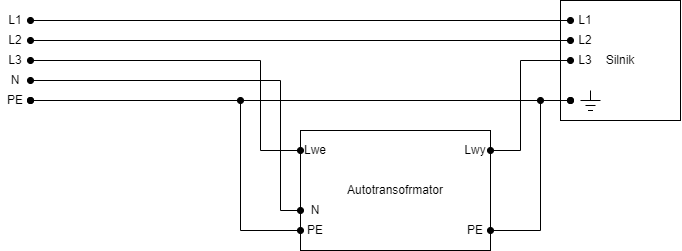
\includegraphics[width=0.9\linewidth]{assets/circut}
	\caption{Schemat połączenia stanowiska badawczego}
	\label{fig:circut}
\end{figure}

\section{Porównanie synchronicznego rejestratora drgań z pomiarem wzorcowym}
By sprawdzić poprawność działania synchronicznego rejestratora drgań, przeprowadzono badanie porównawcze. Pomiarem wzorcowym był sygnał uzyskany z laserowego czujnika położenia. Jako, że SRD (synchroniczny rejestrator drgań) zbiera dane na temat przyspieszeń obiektu w czasie, a laserowy czujnik położenia obiektu w czasie, należało przeprowadzić podwójne różniczkowanie otrzymanych wyników z sygnału wzorcowego, co pozwala na porównanie dwóch jednakowych wielkości fizycznych. 
Blokowy schemat stanowiska badawczego został przedstawiony na Rysunku~\ref{fig:wibro1}. 
\begin{figure}[th]
	\centering
	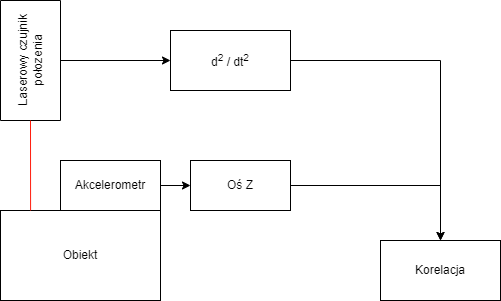
\includegraphics[width=0.8\linewidth]{assets/wibro1.drawio}
	\caption{Schemat blokowy stanowiska badawczego wraz ze sprzętem badawczym}
	\label{fig:wibro1}
\end{figure}


Rysunek~\ref{fig:img20221108124622} przedstawia sposób zamontowania elementów pomiarowych na stanowisku badawczym. Oba elementy pomiarowe posiadają takie same kierunki oraz zwroty w przestrzeni kartezjańskiej.
\begin{figure}[H]
	\centering
	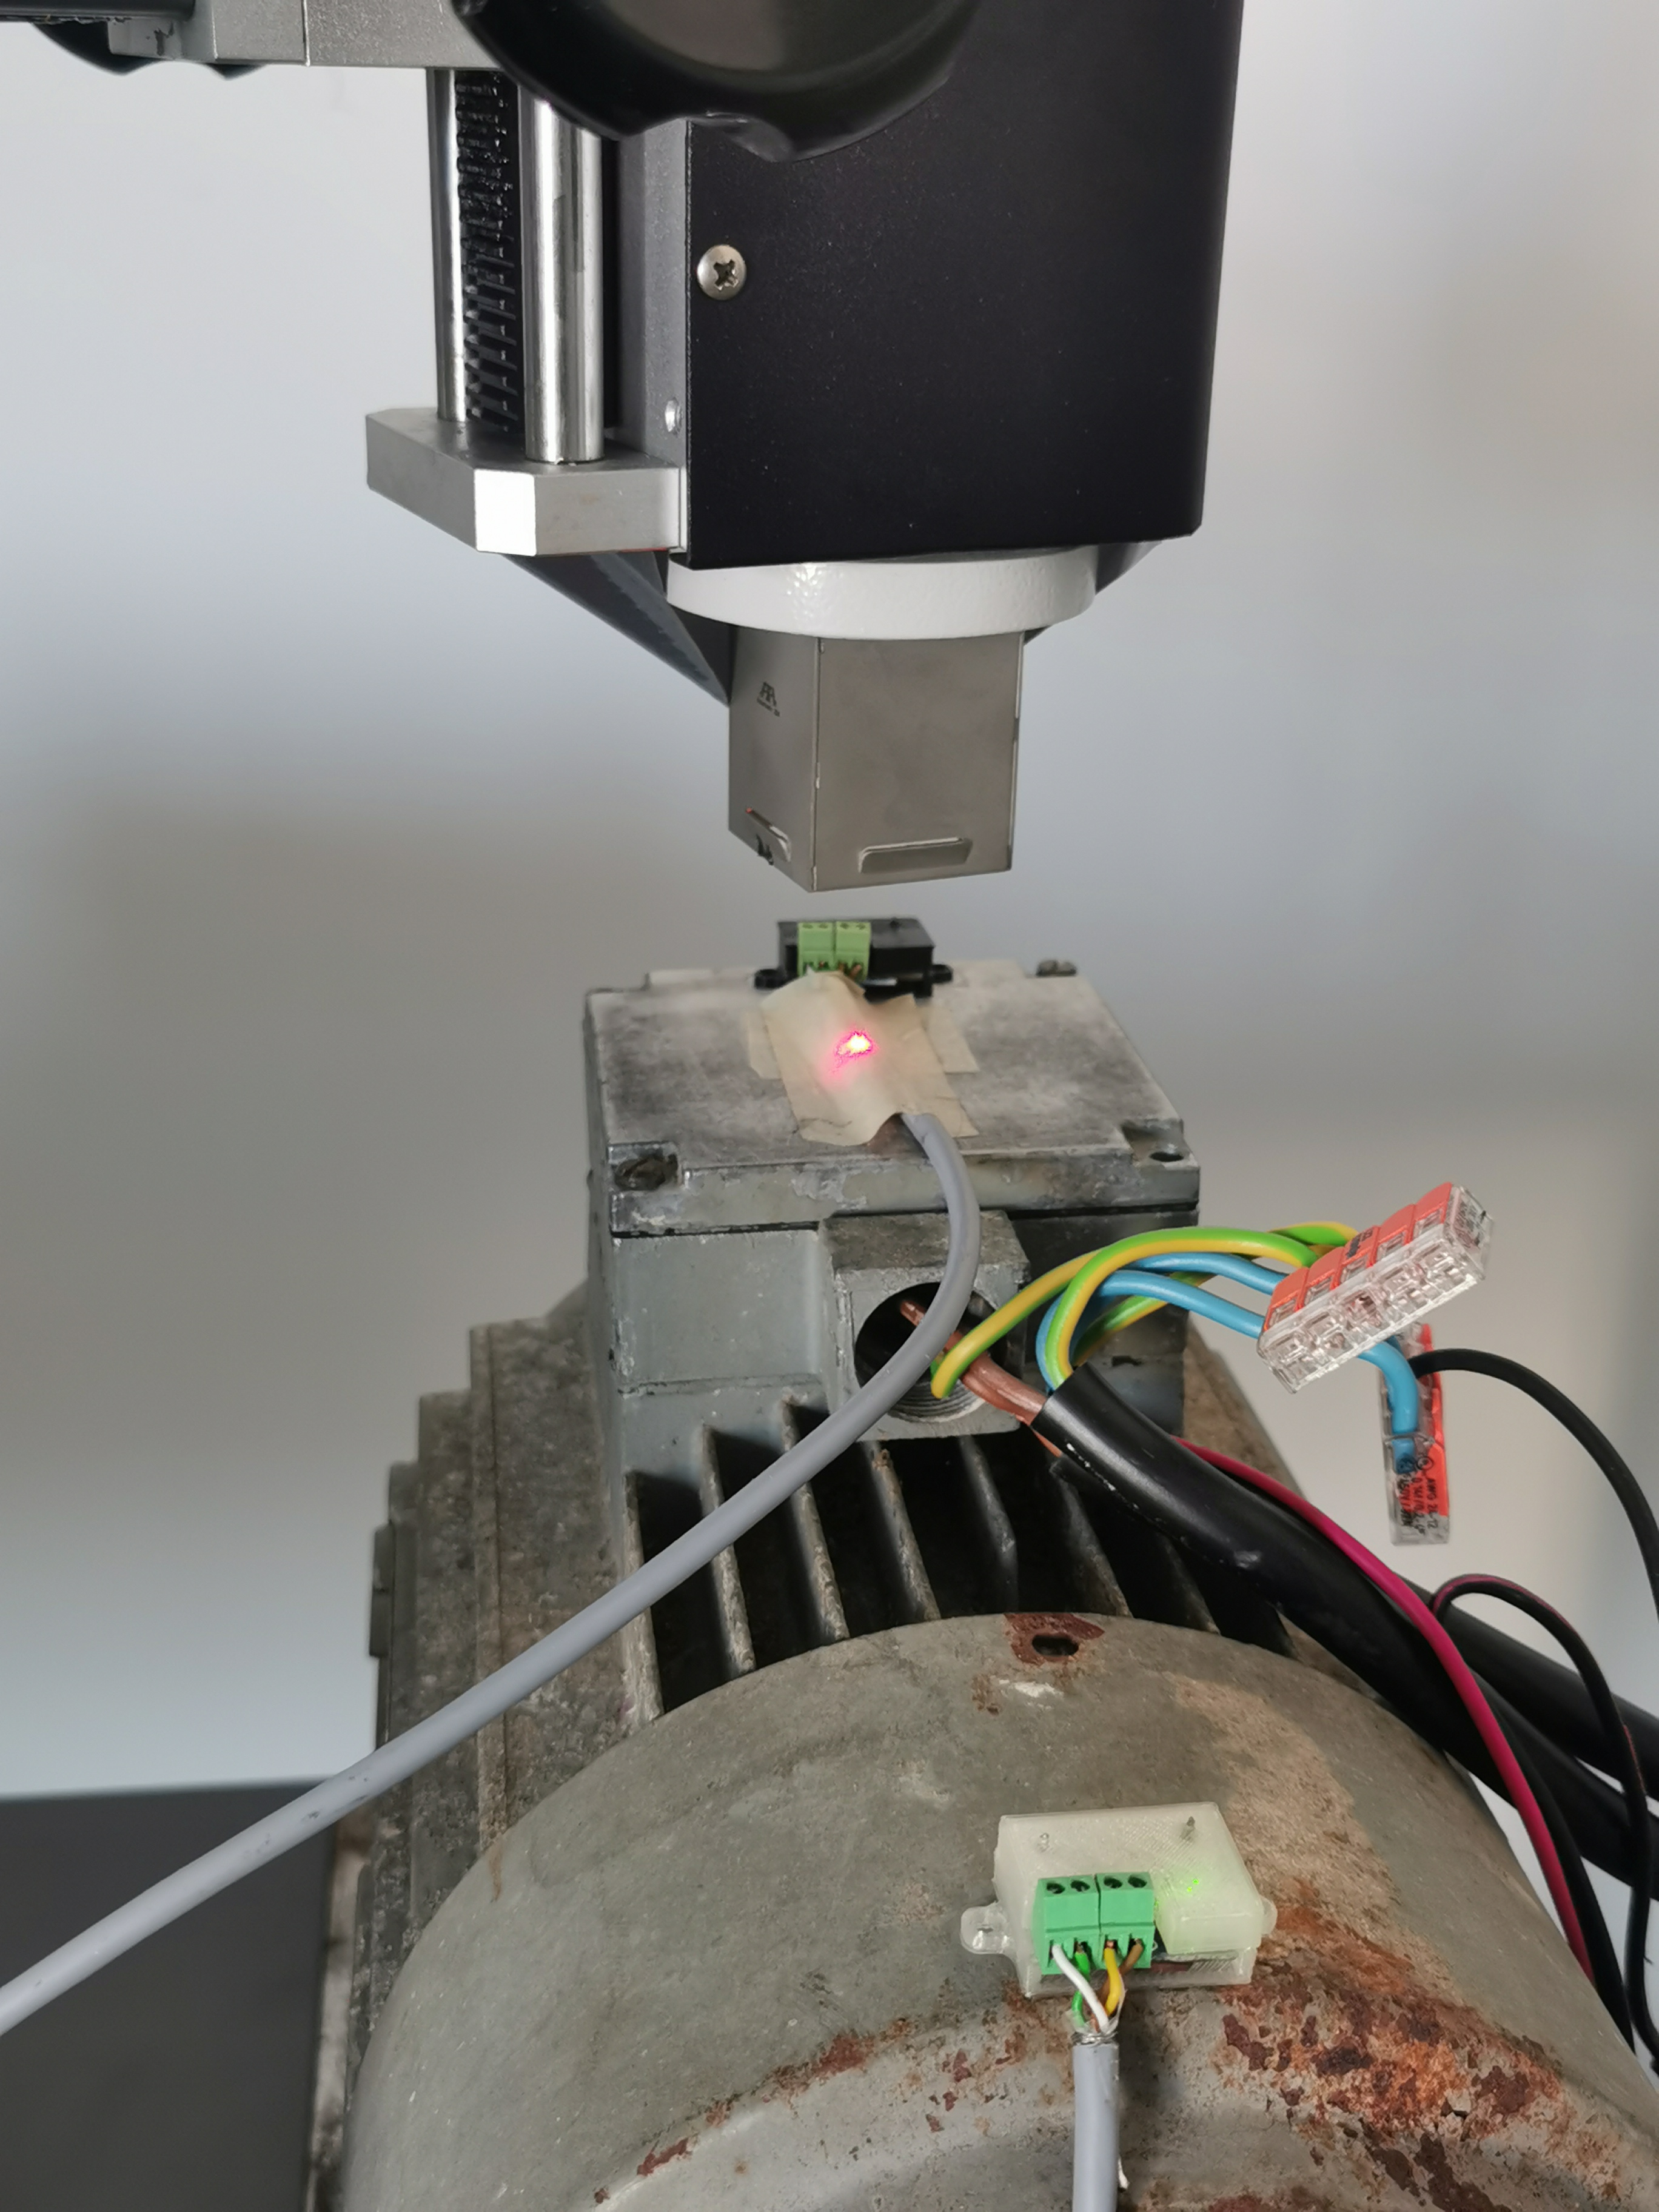
\includegraphics[width=0.6\linewidth]{assets/IMG_20221108_124622}
	\caption{Czujnik położenia oraz SRD zamontowany na obiekcie badawczym.}
	\label{fig:img20221108124622}
\end{figure}
 

\begin{figure}[H]
	\centering
	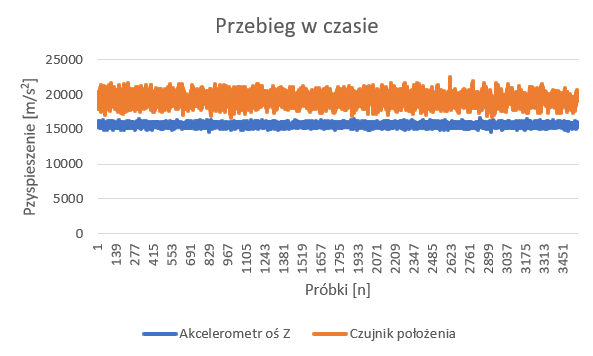
\includegraphics[width=0.95\linewidth]{assets/timePlot1}
	\caption{Przebiegi czasowe otrzymane z obu czujników. Niebieski - akcelerometr, pomarańczowy - czujnik położenia}
	\label{fig:timeplot1}
\end{figure}

\begin{figure}[H]
	\centering
	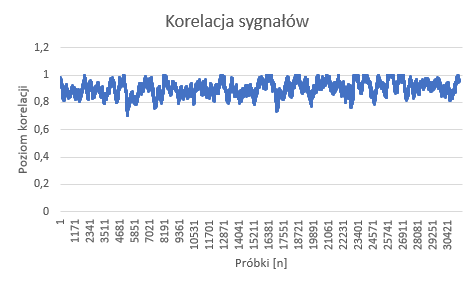
\includegraphics[width=0.9\linewidth]{assets/korelacja1}
	\caption{Korelacja sygnałów otrzymanych z czujnika położenia oraz SRD}
	\label{fig:korelacja1}
\end{figure}

%\newpage
\section{Pomiar w innym kierunku niż orientacja wybranego czujnika układu pomiarowego}
Drugim przeprowadzonym badaniem było porównanie otrzymanych wyników z wzorcowego czujnika oraz testowanego urządzenia. Badanie polegało na tym, że czujnik położenia zostanie skierowany pod pewnym kątem $\theta$ oraz $\gamma$, a następnie otrzymane w ten sposób sygnały zostaną ze sobą porównane poprzez korelacje. Rysunek~\ref{fig:img20221108124849} przedstawia proces zbierania danych.
\begin{figure}[th!]
	\centering
	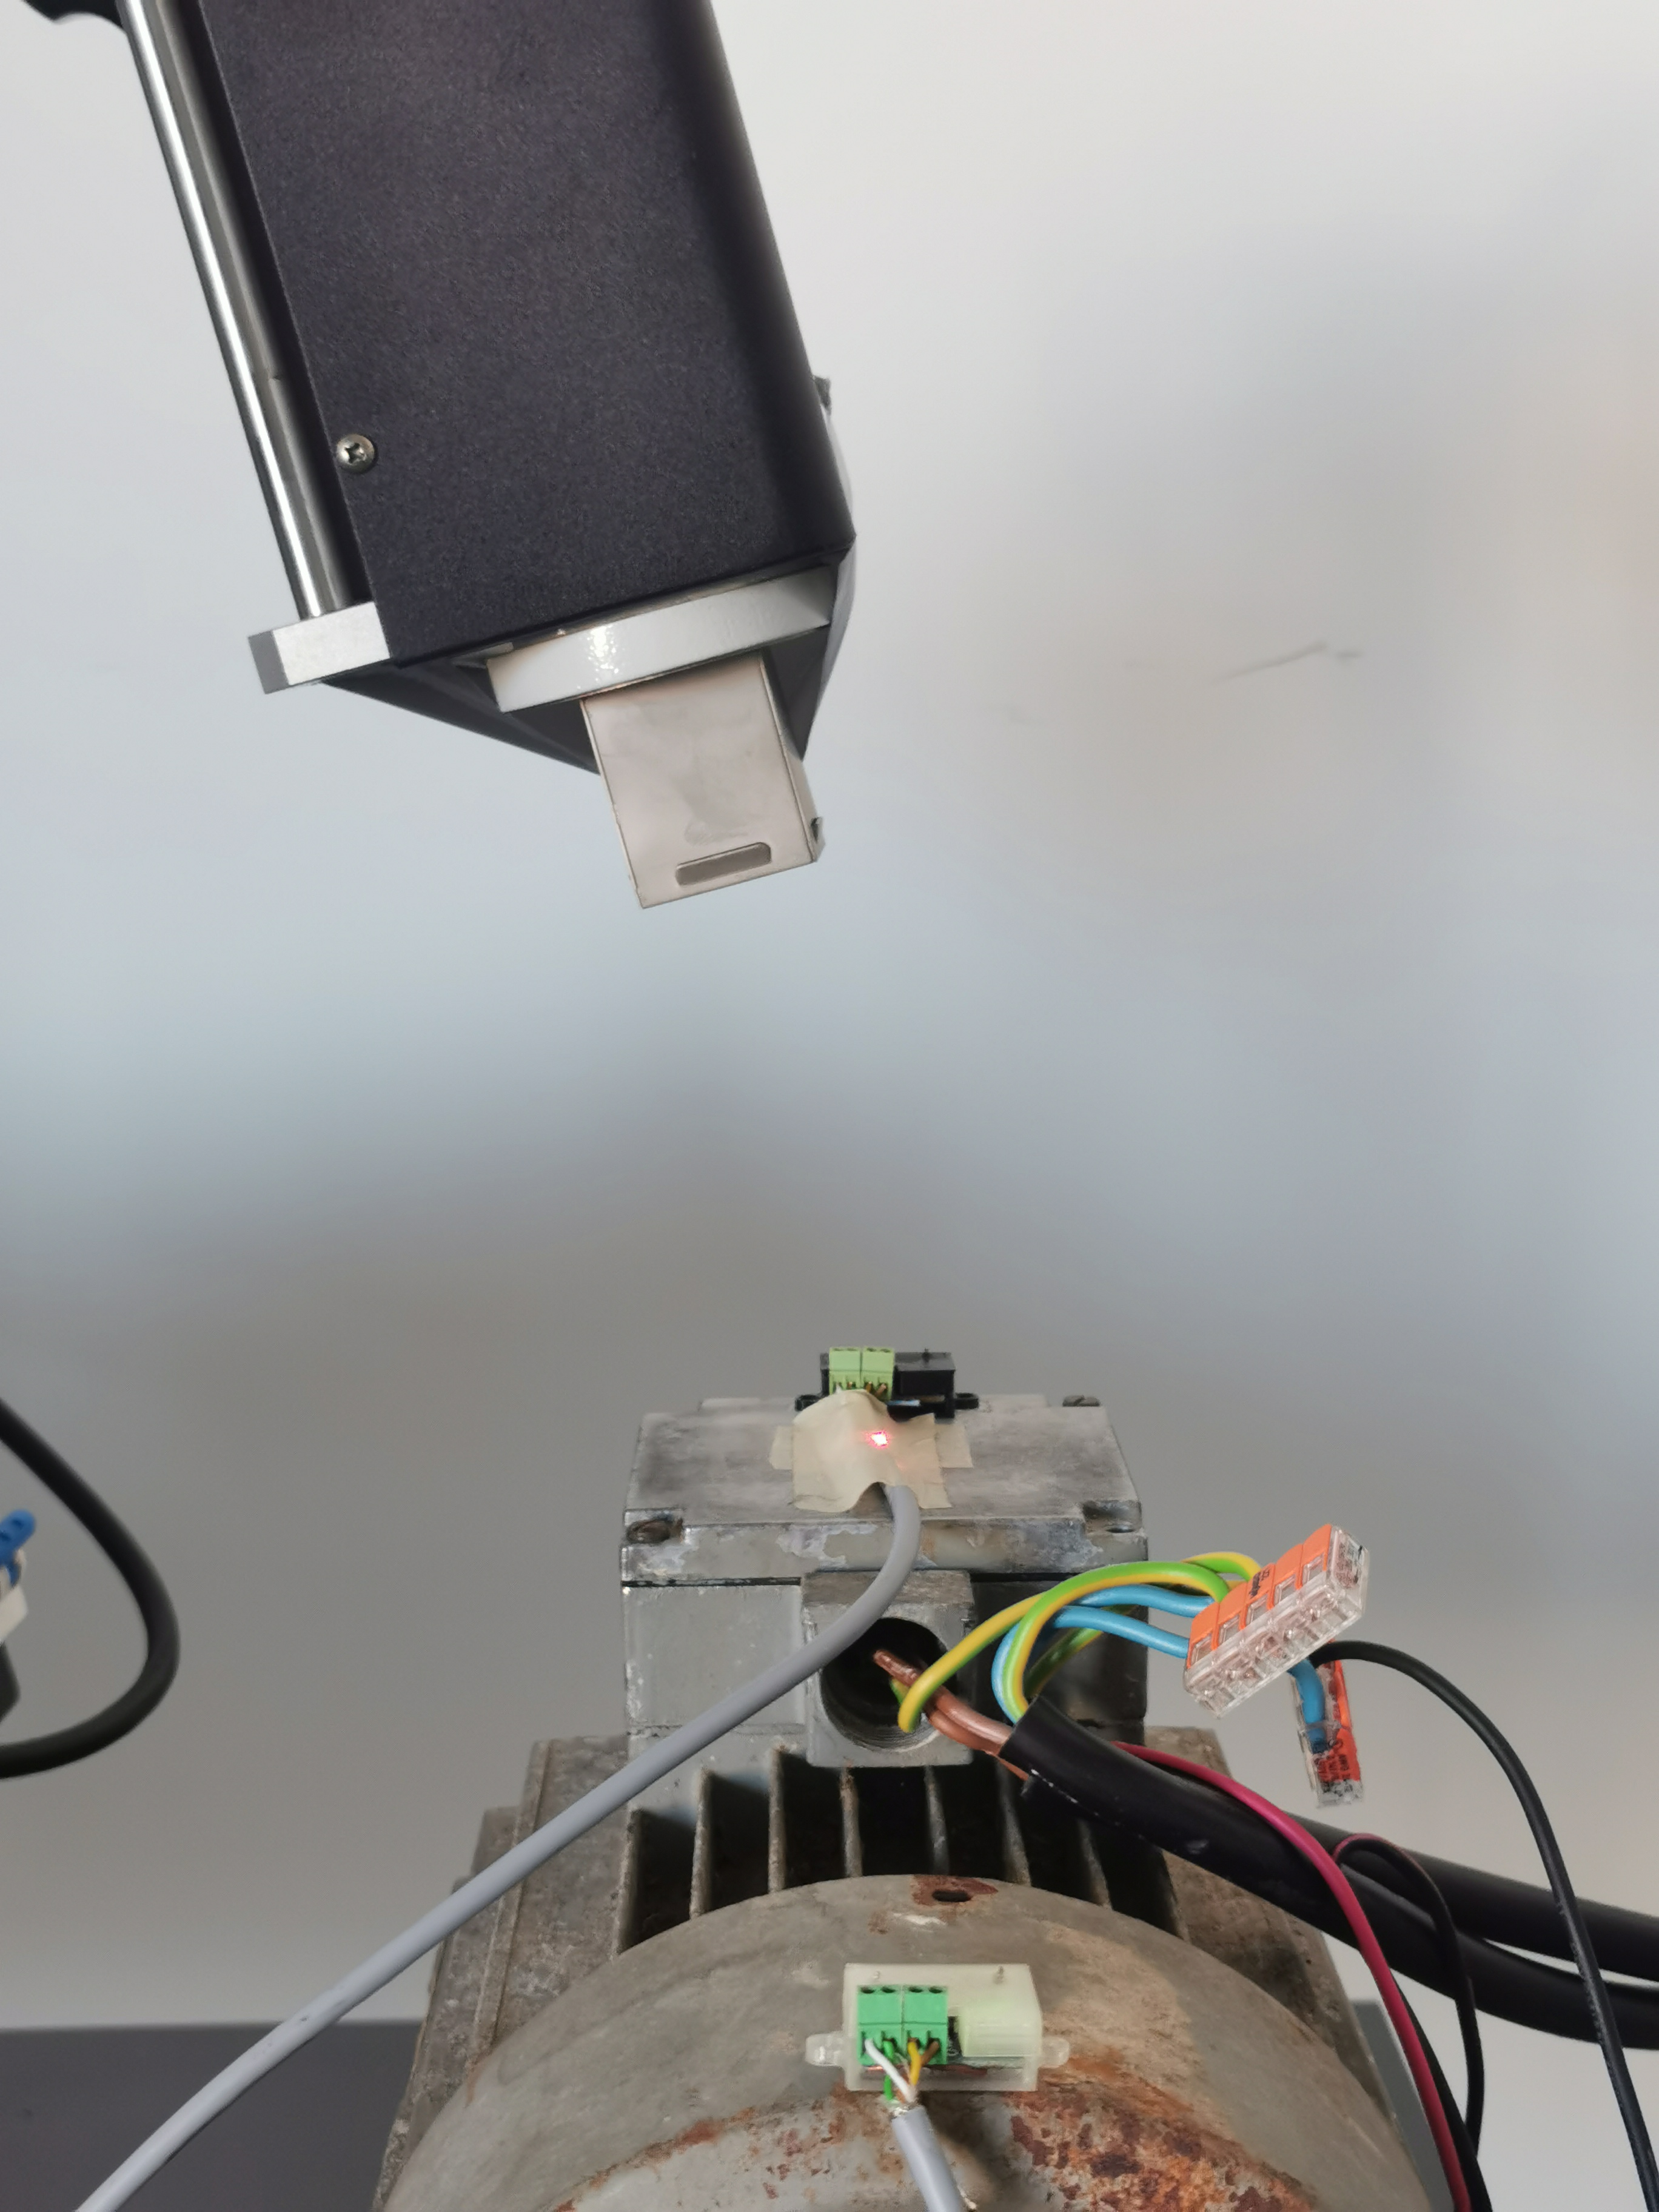
\includegraphics[width=0.7\linewidth]{assets/IMG_20221108_124849}
	\caption{Proces zbierania danych ze stanowiska badawczego, gdy czujnik położenia nachylony jest pod kątem $\theta$ oraz $\gamma$ do badanego obiektu}
	\label{fig:img20221108124849}
\end{figure}

Tak samo jak w pierwszym badaniu by porównać dane otrzymane z dwóch czujników, przeprowadzono podwójne różniczkowane sygnału otrzymanego z czujnika położenia. Jako, że czujnik położenia znajdował się w pewnym nachyleniu do obiektu badawczego, dane z akcelerometru musiały zostać obrócone o wartość wektora $ \begin{pmatrix}0,25 & 0,25 & 1\end{pmatrix} $. Schemat blokowy stanowiska badawczego przedstawia Rysunek~\ref{fig:wibro2}.



\begin{figure}[th]
	\centering
	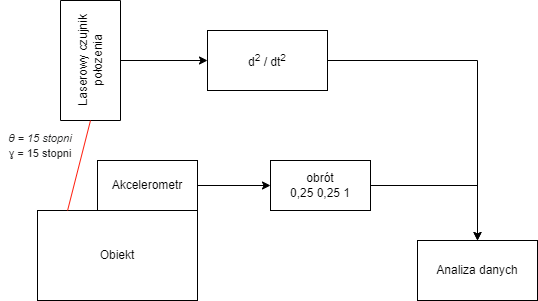
\includegraphics[width=0.9\linewidth]{assets/wibro2}
	\caption{Schemat blokowy stanowiska badawczego wraz ze sprzętem badawczym gdy czujnik położenia jest nachylony do obiektu badawczego}
	\label{fig:wibro2}
\end{figure}


\begin{figure}[h]
	\centering
	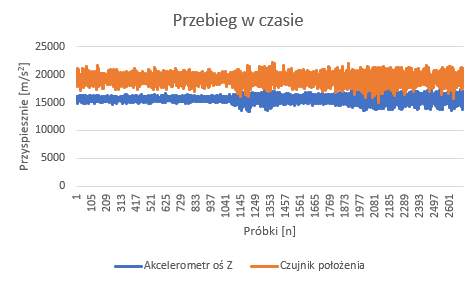
\includegraphics[width=0.9\linewidth]{assets/timePlot2}
	\caption{Przebieg czasowy}
	\label{fig:timeplot2}
\end{figure}

\begin{figure}[h]
	\centering
	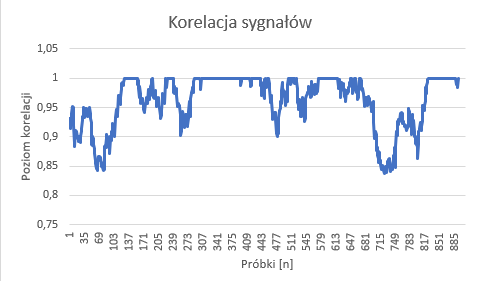
\includegraphics[width=0.9\linewidth]{assets/korelacja2}
	\caption{Korelacja sygnałów}
	\label{fig:korelacja2}
\end{figure}



\end{document}
